\documentclass[a4paper,11pt]{ujreport}
%%【PostScript, JPEG, PNG等の画像の貼り込み】
%% 利用するパッケージを選んでコメントアウトしてください.
\usepackage{graphicx} % for 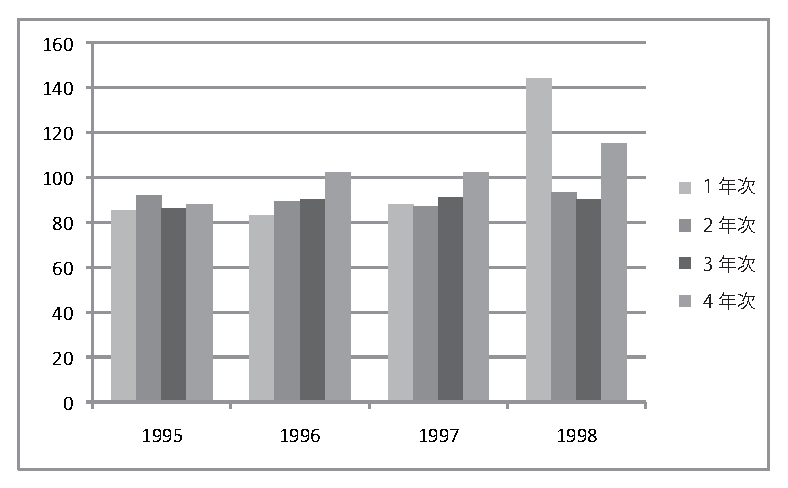
\includegraphics[width=3cm]{sample.eps}
\usepackage{epsfig} % for 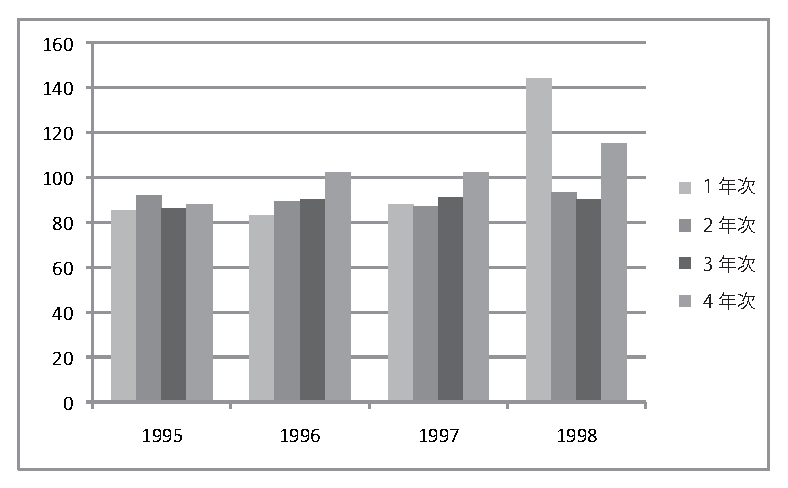
\psfig{file=sample.eps,width=3cm}
%\usepackage{epsf} % for \epsfile{file=sample.eps,scale=0.6}
%\usepackage{epsbox} % for \epsfile{file=sample.eps,scale=0.6}
\usepackage{/Users/takagihayata/workspace/materialize-mongodb/paper/mast/class/mediabb} % for pdf

\usepackage{times} % use Times Font instead of Computer Modern
% \usepackage{listings} % for soursecode
% \usepackage{plistings} % for soursecode
\usepackage{/Users/takagihayata/workspace/materialize-mongodb/paper/mast/class/docmute} % texファイル分割用

\setcounter{tocdepth}{3}
\setcounter{page}{-1}

\setlength{\oddsidemargin}{0.1in}
\setlength{\evensidemargin}{0.1in}
\setlength{\topmargin}{0in}
\setlength{\textwidth}{6in}
%\setlength{\textheight}{10.1in}
\setlength{\parskip}{0em}
\setlength{\topsep}{0em}

%\newcommand{\zu}[1]{{\gt \bf 図\ref{#1}}}

%% タイトル生成用パッケージ(重要)
\usepackage{/Users/takagihayata/workspace/materialize-mongodb/paper/mast/class/mast-jp-sjis}

%% タイトル
%% 【注意】タイトルの最後に\\ を入れるとエラーになります
\title{NoSQL型データベースシステムでの実体化ビュー選択に関する研究}
%% 著者
\author{髙木 颯汰}
%% 指導教員
\advisor{古瀬 一隆 陳 漢雄}

%% 年月 (提出年月)
%% 年月は必要に応じて書き替えてください.
\majorfield{ } \yearandmonth{2019年 1月}


\addtocounter{page}{2} %単体でコンパイルした際の調整用
\addtocounter{chapter}{0} %単体でコンパイルした際の調整用
\begin{document}

\chapter{はじめに}
\label{chap:Introduction}

数年前までは主要なデータストアとして,リレーショナルデータベースがあげられることがほとんどであった.それは多くの開発者がSQLに慣れ親しんでおり,正規化されたデータモデル,トランザクションの必要性,耐久性のあるストレージエンジンが提供する保証を受けられるからである\cite{Sky株式会社201212}.しかし近年高いスケーラビリティや大量なデータ処理が得意であることなどからNoSQLに対する需要が急激に増えている.

例えばNoSQLの一種のドキュメント指向データベースはデータベースの構造を表すスキーマを定義する必要がなく,大量なデータを事前準備なしで格納することができる.従来のリレーショナルデータベースにあったような参照型のデータ構造に加えて埋込型のデータ構造を選択できる.型宣言の必要のないスクリプト言語と相性が良いことなども合間って,プロトタイプを高速に開発することが求められるビジネスの現場で採用されることが増えている\cite{渡部201602}.

一方でドキュメント指向データベースの特徴とも言える階層的なデータモデルが更新処理速度の低下やデータ参照の柔軟性を低下を招くことがある.これを防ぐためにはドキュメントに階層的に埋め込むフィールドを適切に選択する必要がある.本論文ではこの選択の自動化し,ドキュメント指向データベースのデータモデルのチューニングを行い,データアクセスを高速化する.

本論文の構成は以下の通りである.まず,第\ref{chap:LiteratureReview}章において関連研究について紹介する.次に,第\ref{chap:ProposedAlgorithm}章において本研究の提案手法について説明をし,第\ref{chap:Experiment}章にて提案手法に関する実験を行い,提案手法の有用性を確める.第\ref{chap:Result}章において実験の結果と考察を述べ,最後に第\ref{chap:Conclusion}章において本論文のまとめと今後の課題を示す.

\end{document}
